\newpage
\section{Insurance Risk}

\subsection{Poisson Process}
\begin{definition}[Poisson process]
    A \textbf{Poisson process} $(N_t)_{t\ge0}$ is a counting process with jump size equals to $+1$ only and the path is constant between two jumps. The value of count $N_t$ is defined as:
    \begin{align*}
        N_t = \sum_{k\ge 1}\1{t \ge T_k}
    \end{align*}

    \noindent Where $(T_k)_{k\ge1}$ is an \textbf{increasing jump-time family} such that:
    \begin{align*}
        \lim_{k\to\infty}T_k = +\infty
    \end{align*}
\end{definition}

\begin{figure}[ht]
    \centering
    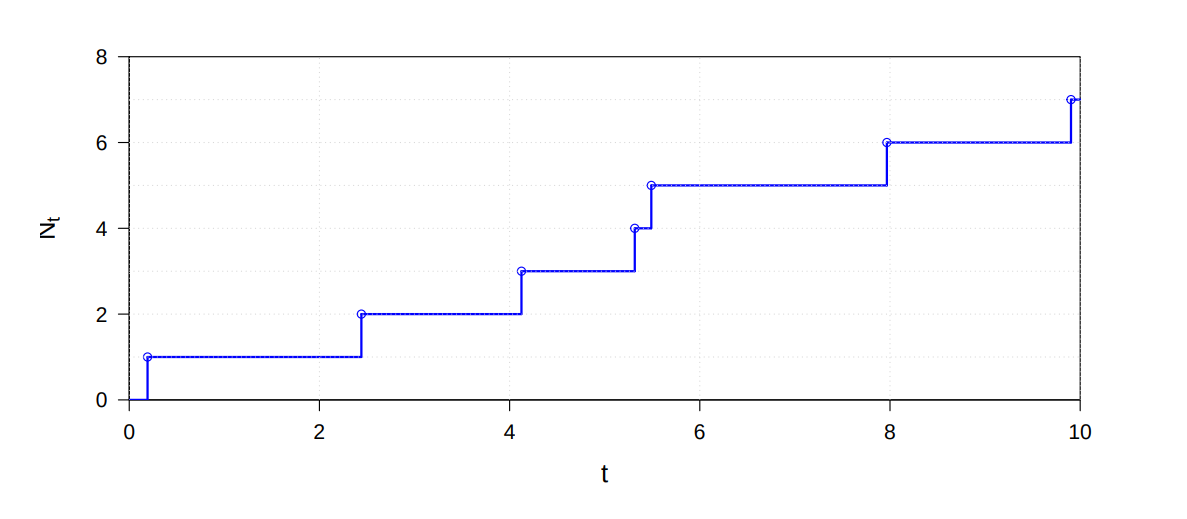
\includegraphics[width=\textwidth]{figures/sample_homogeneous_poisson_process.png}
    \caption{Homogeneous Poisson Process with constant jump size (figure sampled from \cite{book:privault})}
    \label{fig:sample-homogeneous-poisson-proc}
\end{figure}

\begin{proposition}{Properties of Poisson Process}{properties_of_poisson_proc}
    In order for the counting process $(N_t)_{t\ge0}$ to be a Poisson process, it has to satisfy the following properties:
    \begin{itemize}
        \item \textbf{Independence of increments} : For all $0 \le t_0 < t_1 < \dots < t_n$ and $n\ge1$ increments, we have
        \begin{align*}
            N_{t_1} - N_{t_0}, N_{t_2} - N_{t_1}, \dots, N_{t_n} - N_{t_{n-1}}
        \end{align*}
        \noindent are mutually independent random variables.
        \item \textbf{Stationarity of increments} : For all $0 \le s \le t$ and some $h>0$, the increment $N_{t} - N_s$ has the same distribution as $N_{t+h} - N_{s+h}$. In other words, for some $k\ge 0$, we have:
        \begin{align*}
            P(N_{t+h} - N_{s+h} = k) = P(N_t - N_s = k)
        \end{align*}
    \end{itemize}
\end{proposition}

\begin{theorem}{Poisson increment}{poisson_increment}
    Let $(N_t)_{t\ge0}$ be a Poisson process. For any $0 \le s \le t$, the increment $N_t-N_s$ follows a Poisson distribution with parameter $(t-s)\lambda$ for some $\lambda > 0$.
    \begin{align*}
        N_t - N_s \sim Poisson\Big( (t-s)\lambda \Big)
    \end{align*}

    \noindent The constant $\lambda$ is called the \textbf{intensity of Poisson process} $(N_t)_{t\ge0}$ and is given by:
    \begin{align*}
        \lambda = \lim_{h\to 0}\frac{1}{h}P(N_h=1)
    \end{align*}
    \noindent Intuitively, the parameter $\lambda$ reflects how soon it is the get the first count. The higher the intensity, the closer the gap in between jumps.
\end{theorem}
\begin{proof*}[Theorem \ref{thm:poisson_increment}]
    (The proof for theorem \ref{thm:poisson_increment} is too technical and will not be included. Refer to \cite{book:Bosq1996} for more information).
\end{proof*}

\begin{corollary}{Distribution of $N_t$}{distribution_of_nt}
    As a direct consequence of theorem \ref{thm:poisson_increment}, we have:
    \begin{align*}
        N_t\sim Poisson\Big( \lambda t \Big) \implies P(N_t = k) = \frac{(\lambda t)^ke^{-\lambda t}}{k!}
    \end{align*}
\end{corollary}

\begin{corollary}{Short-time asymptotics of Poisson process}{short_time_behaviour_poisson_proc}
    For a current state $N_t$ of the Poisson process, the behaviour of the process in a short time $h>0$ ahead is expressed in the following probability:
    \begin{align*}
        P(N_{t+h} - N_t) \approx \frac{\lambda^kh^k}{k!}, \ h \to 0
    \end{align*}
\end{corollary}
\begin{proof*}[Corollary \ref{coro:short_time_behaviour_poisson_proc}]
    By theorem \ref{thm:poisson_increment}, we have:
    \begin{align*}
        N_{t+h} - N_t \sim Poisson(h\lambda)
    \end{align*}

    \noindent Hence, we have:
    \begin{align*}
        P(N_{t+h} - N_t) &= \frac{(\lambda h)^k e^{-\lambda h}}{k!} \\
        &\approx \frac{\lambda^kh^k}{k!} \ \ \text{(When $h\approx 0$)}
    \end{align*}

    \noindent Because $e^{-\lambda h} \to 1$ as $h \to 0$.
\end{proof*}

\begin{proposition}{Distribution of jump-time $T_n$}{jump_time_distribution}
    For all $n\ge1$, the jump-time $T_n$ has the gamma distribution:
    \begin{align*}
        T_n \sim Gamma(n, 1/\lambda)
    \end{align*}

    \noindent With the probability density function:
    \begin{align*}
        f_{T_n}(t) = \lambda^n e^{-\lambda t}\frac{t^{n-1}}{(n-1)!} = \lambda^n e^{-\lambda t}\frac{t^{n-1}}{\Gamma(n)}
    \end{align*}
    \noindent For all $t>0$, the probability that $T_n\ge t$ is given by:
    \begin{align*}
        P(T_n \ge t) = \lambda^n \int_t^\infty e^{-\lambda s}\frac{s^{n-1}}{(n-1)!}ds
    \end{align*}
\end{proposition}
\begin{proof*}[Proposition \ref{prop:jump_time_distribution}]
    Proving by induction, for base case, we have:
    \begin{align*}
        P(T_1 \ge t) = P(T_1 > t) = P(N_t = 0) = e^{-\lambda t}
    \end{align*}

    \noindent For inductive case, suppose that we have:
    \begin{align*}
        P(T_{n-1} > t) = \lambda^{n-1}\int_{t}^{\infty} e^{-\lambda s}\frac{s^{n-2}}{(n-2)!}ds
    \end{align*}

    \noindent For $T_n$, we have:
    \begin{align*}
        P(T_n > t) &= P(T_n > t \ge T_{n-1}) + P(T_{n-1}>t) \\
        &= P(N_t = n-1) + P(T_{n-1} > t) \\
        &= \frac{(\lambda t)^{n-1} e^{-\lambda t}}{(n-1)!} + \lambda^{n-1}\int_{t}^{\infty} e^{-\lambda s}\frac{s^{n-2}}{(n-2)!}ds \\
        &= \lambda \int_{t}e^{-\lambda s}\frac{(\lambda s)^{n-1}}{(n-1)!}ds \\
        &= \lambda ^n\int_t^\infty \frac{e^{-\lambda s}s^{n-1}}{(n-1)!}ds
    \end{align*}
\end{proof*}

\subsection{Compound Poisson Process}
\begin{definition}[Compound Poisson Process]
    Let $(Z_k)_{k\ge1}$ be a sequence of i.i.d square integrable random variables with a probability distribution $\nu(.)$ independent of the Poisson Process $(N_t)_{t\ge0}$.

    \noindent\newline The process $(Y_t)_{t\ge0}$ is called a \textbf{Compound Poisson Process} if it is given by the random sum:
    \begin{align*}
        Y_t = \sum_{k=1}^{N_t}Z_k
    \end{align*}

    \noindent The Compound Poisson Process is indeed a Poisson process because it satisfies both properties:
    \begin{itemize}
        \item \textbf{Independent increments}.
        \item \textbf{Stationarity of increments}.
    \end{itemize}
\end{definition}

\begin{figure}[ht]
    \centering
    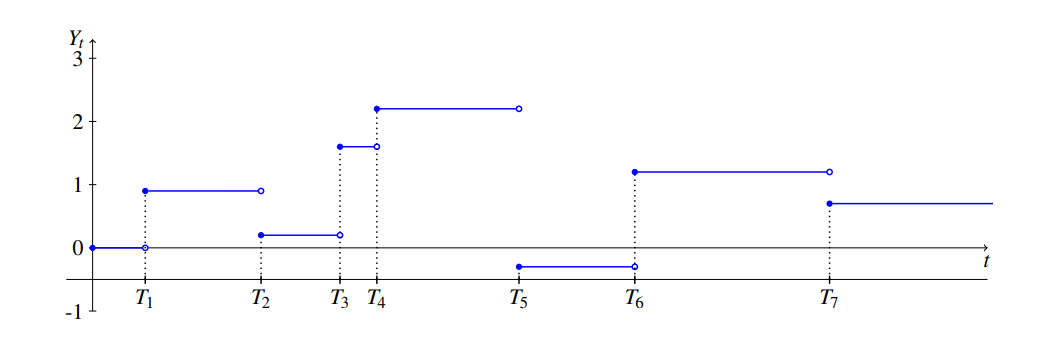
\includegraphics[width=\textwidth]{figures/sample_compound_poisson_process.png}
    \caption{Compound Poisson Process with non-constant jump size (figure sampled from \cite{book:privault})}
    \label{fig:sample-compound-poisson-process}
\end{figure}

\begin{proposition}{Mean and Variance of $(Y_t)_{t\ge0}$}{mean_var_of_comp_poisson_proc}
    Let $\mathbb{E}\Big[ N_t \Big]$ be the mean number of jump times and $\mathbb{E}\Big[Z\Big]$ be the mean jump size. We have:
    \begin{itemize}
        \item $\mathbb{E}[Y_t] = \mathbb{E}[N_t]\mathbb{E}[Z] = \lambda t\mathbb{E}[Z]$.
        \item $Var(Y_t) = \mathbb{E}[N_t] \mathbb{E}[Z^2] = \lambda t \mathbb{E}[Z^2]$.
    \end{itemize}
\end{proposition}

\subsection{Claim and Reserve Process}
\textbf{Overview} : In an insurance risk settings, we have
\begin{itemize}
    \item \textbf{Number of claims $(N_t)$} : modelled by the homogeneous (constant jump size) Poisson process $(N_t)_{t\ge0}$ with intensity $\lambda > 0$.
    \item \textbf{Claim amounts $(Z_k)$} : A sequence of non-negative, i.i.d random variables.
\end{itemize}

\begin{definition}[Aggregated claims]
    The \textbf{Aggregated claim} amount up to time $t$ is defined by the Compound Poisson Process:
    \begin{align*}
        S(t) = \sum_{k=1}^{N_t} Z_k
    \end{align*}
\end{definition}

\begin{definition}[Standard compound risk model]
    The reserve process is defined by
    \begin{align*}
        R_x(t) = x + f(t) - S(t)
    \end{align*}

    \noindent Where $x\ge0$ is the initial reserve, $f(t)$ is an income function up to time $t>0$ and $S(t)$ is the aggregated claims. 
\end{definition}

\begin{figure}[ht]
    \centering
    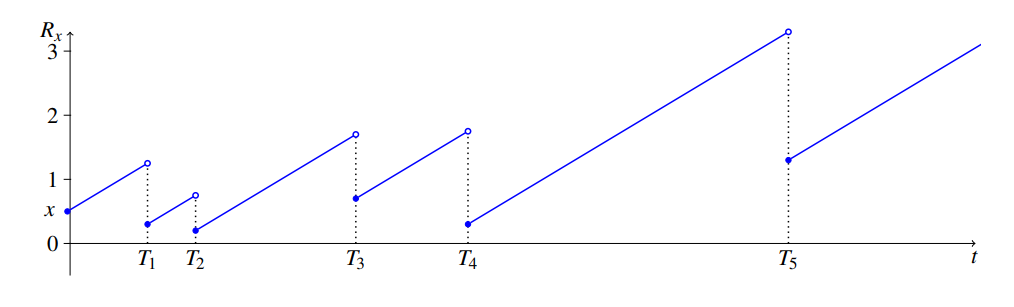
\includegraphics[width=\textwidth]{figures/sample_reserve_process.png}
    \caption{Sample reserve process with non-zero initial reserve and a linear income function (figure sampled from \cite{book:privault})}
    \label{fig:sample-reserve-process}
\end{figure}

\subsection{Ruin Probability}
\begin{definition}[Ruin probability]
    There are two types of ruin probabilities
    \begin{itemize}
        \item \textbf{Infinite-time ruin probability} :
        \begin{align*}
            \Psi(x) = P(\exists t \in [0, \infty) : R_x(t) < 0)
        \end{align*}

        \item \textbf{Finite-time ruin probability} :
        \begin{align*}
            \Psi_T(x) = P(\exists t \in [0, T]:R_x(t) < 0)
        \end{align*}
    \end{itemize}
\end{definition}

\begin{theorem}{Cramer Lundberg model}{cramer_lundberg}
    Assume that the income function is linear with a positive slope $f(t) = ct$. We have:
    \begin{itemize}
        \item \textbf{Zero initial reserve} : 
        \begin{align*}
            \Psi(x) = \frac{\lambda\mu}{c}
        \end{align*}
        \noindent Provided that $c > \lambda\mu$ where $\mu = \mathbb{E}[Z]$. 

        \item \textbf{Non-zero initial reserve} : Suppose that $Z_k \sim Exponential(1/\mu)$. then,
        \begin{align*}
            \Psi(x) = \frac{\lambda \mu}{c}\exp\Bigg(\Bigg( \frac{\lambda}{c} - \frac{1}{\mu} \Bigg)x\Bigg)
        \end{align*}
    \end{itemize}

    \noindent Either case, $\Psi(x)=1$ if $c \le \lambda \mu$.
\end{theorem}

